\section{Eigenfunctions of CT systems}
To summarize the course so far given an input signal $x(t)$ and a LTI system described (equivalently) by a linear, constant coefficient differential equation, impulse response, or a block diagram, we can determine the output using convolution. This is referred to as \emph{time-domain} analysis.

The advantages of this approach are that the analysis is straightforward (if cumbersome) and it applies to all LTI systems, stable or otherwise. Time-domain representations of signals are also intuitive given their direct application in physical systems.

There are also some disadvantages. First, time-domain analysis does not scale well to larger systems since analysis with block diagram decompositions requires convolution, and in the case of the feedback motif dealing with inverse systems or de-convolution. Second, it is difficult to design an impulse responses for a given purpose. Finally implementing a system directly from an impulse response is not intuitive.

We can borrow a technique from mathematics to overcome these disadvantages by transforming the \emph{domain} of the representations to one in which the operation of convolution becomes one of multiplication. This approach, called generally \emph{frequency domain} analysis has a number of advantages and will be our focus for the remainder of the course.

\subsection{The Response of LTI Systems to Complex Exponentials}

Recall convolution can be viewed as a decomposition of a signal into an infinite sum of $\delta$ functions plus the linearity property.
\[
x(t) = \int\limits_{-\infty}^{\infty} x(\tau)\delta(t-\tau) \; d\tau \;\longrightarrow\; y(t) = \int\limits_{-\infty}^{\infty} x(\tau)h(t-\tau) \; d\tau
\]
  
We now consider a different decomposition based on the complex exponential, $e^{st}$ for $s \in \mathbb{C}$, rather than $\delta$ functions. As we will see this decomposition simplifies convolution, turning it into multiplication.

\subsubsection{Eigenfunction $e^{st}$ and Transfer Function $H(s)$}

Let $x(t) = e^{st}$ for $s\in \mathbb{C}$, then $y(t) = h(t) * x(t) = x(t) * h(t)$ and by the definition of convolution
\begin{align*}
  y(t) & = \int\limits_{-\infty}^{\infty}h(\tau)x(t-\tau)\; d\tau\\
  &= \int\limits_{-\infty}^{\infty}h(\tau)e^{s(t-\tau)}\; d\tau = \int\limits_{-\infty}^{\infty}h(\tau)e^{st}e^{-s\tau}\; d\tau\\
  &= e^{st} \int\limits_{-\infty}^{\infty}h(\tau)e^{-s\tau}\; d\tau\\
  &= e^{st}H(s)
\end{align*}
where $H(s) = \int\limits_{-\infty}^{\infty}h(\tau)e^{-s\tau}\; d\tau$ is the \emph{Laplace Transform} of the impulse response, $h(t)$. $H(s)$ is called the \emph{transfer function} or \emph{Eigenvalue} of the system and $e^{st}$ is the \emph{Eigenfunction} for CT LTI systems.

Similar to the impulse function, the complex exponential is a special signal because it's response is easy to determine. It is just the same signal scaled by a multiplicative factor as illustrated below:

\begin{center}
  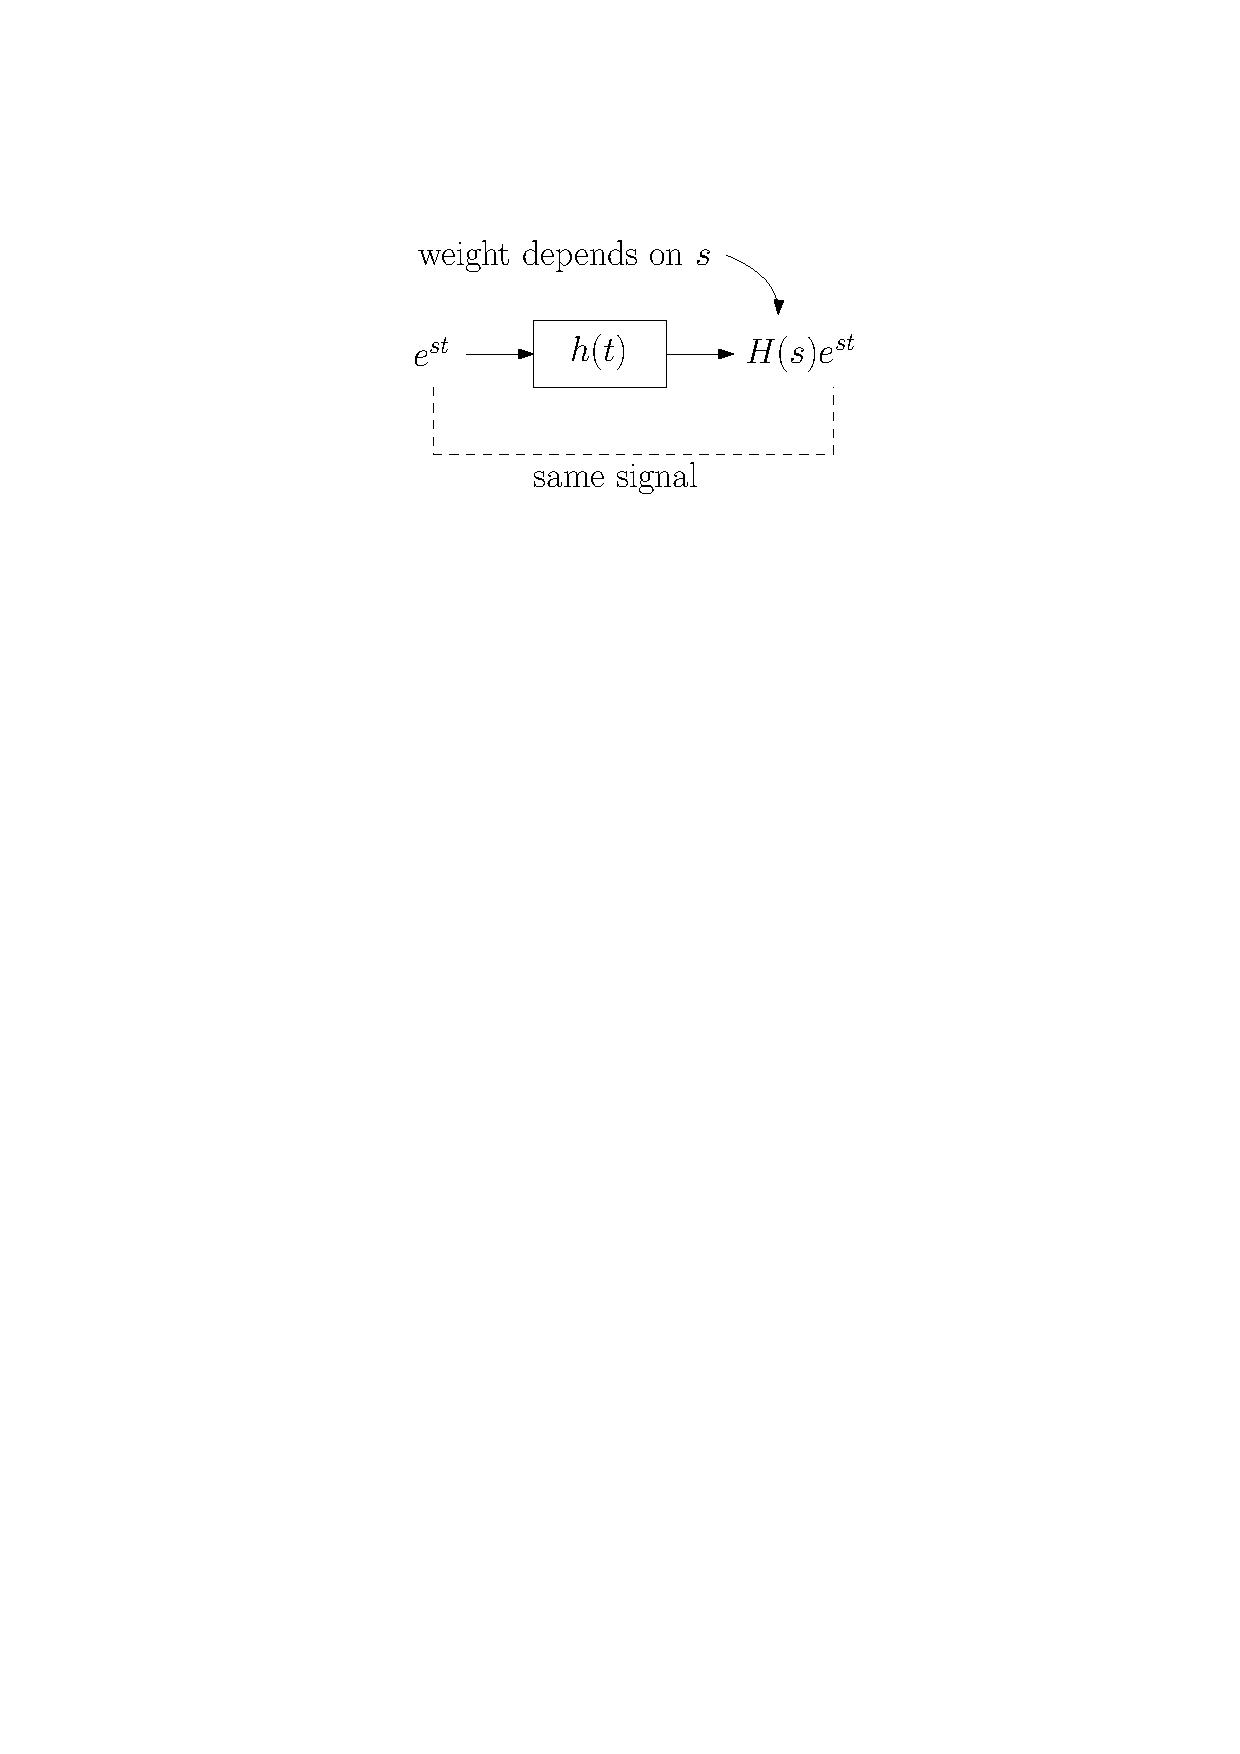
\includegraphics[scale=0.6]{graphics/lti-ct-complex-exp.pdf}
\end{center}

\begin{example}
Suppose $H(s) = \frac{1}{s+1}$ and $x(t) = e^{(-4+j2\pi)t}$. Then the output is
\begin{align*}
  y(t) &= H(-4+j2\pi)e^{(-4+j2\pi)t}\\
  &= \frac{1}{-4+j2\pi+1}e^{(-4+j2\pi)t}\\
  &= \frac{1}{-3+j2\pi}e^{(-4+j2\pi)t} \; ,
\end{align*}
another complex exponential.\\
$\blacksquare$
\end{example}

Given $H(s)$ and inputs that are sums of complex exponentials, the output is easy to determine.

\begin{center}
  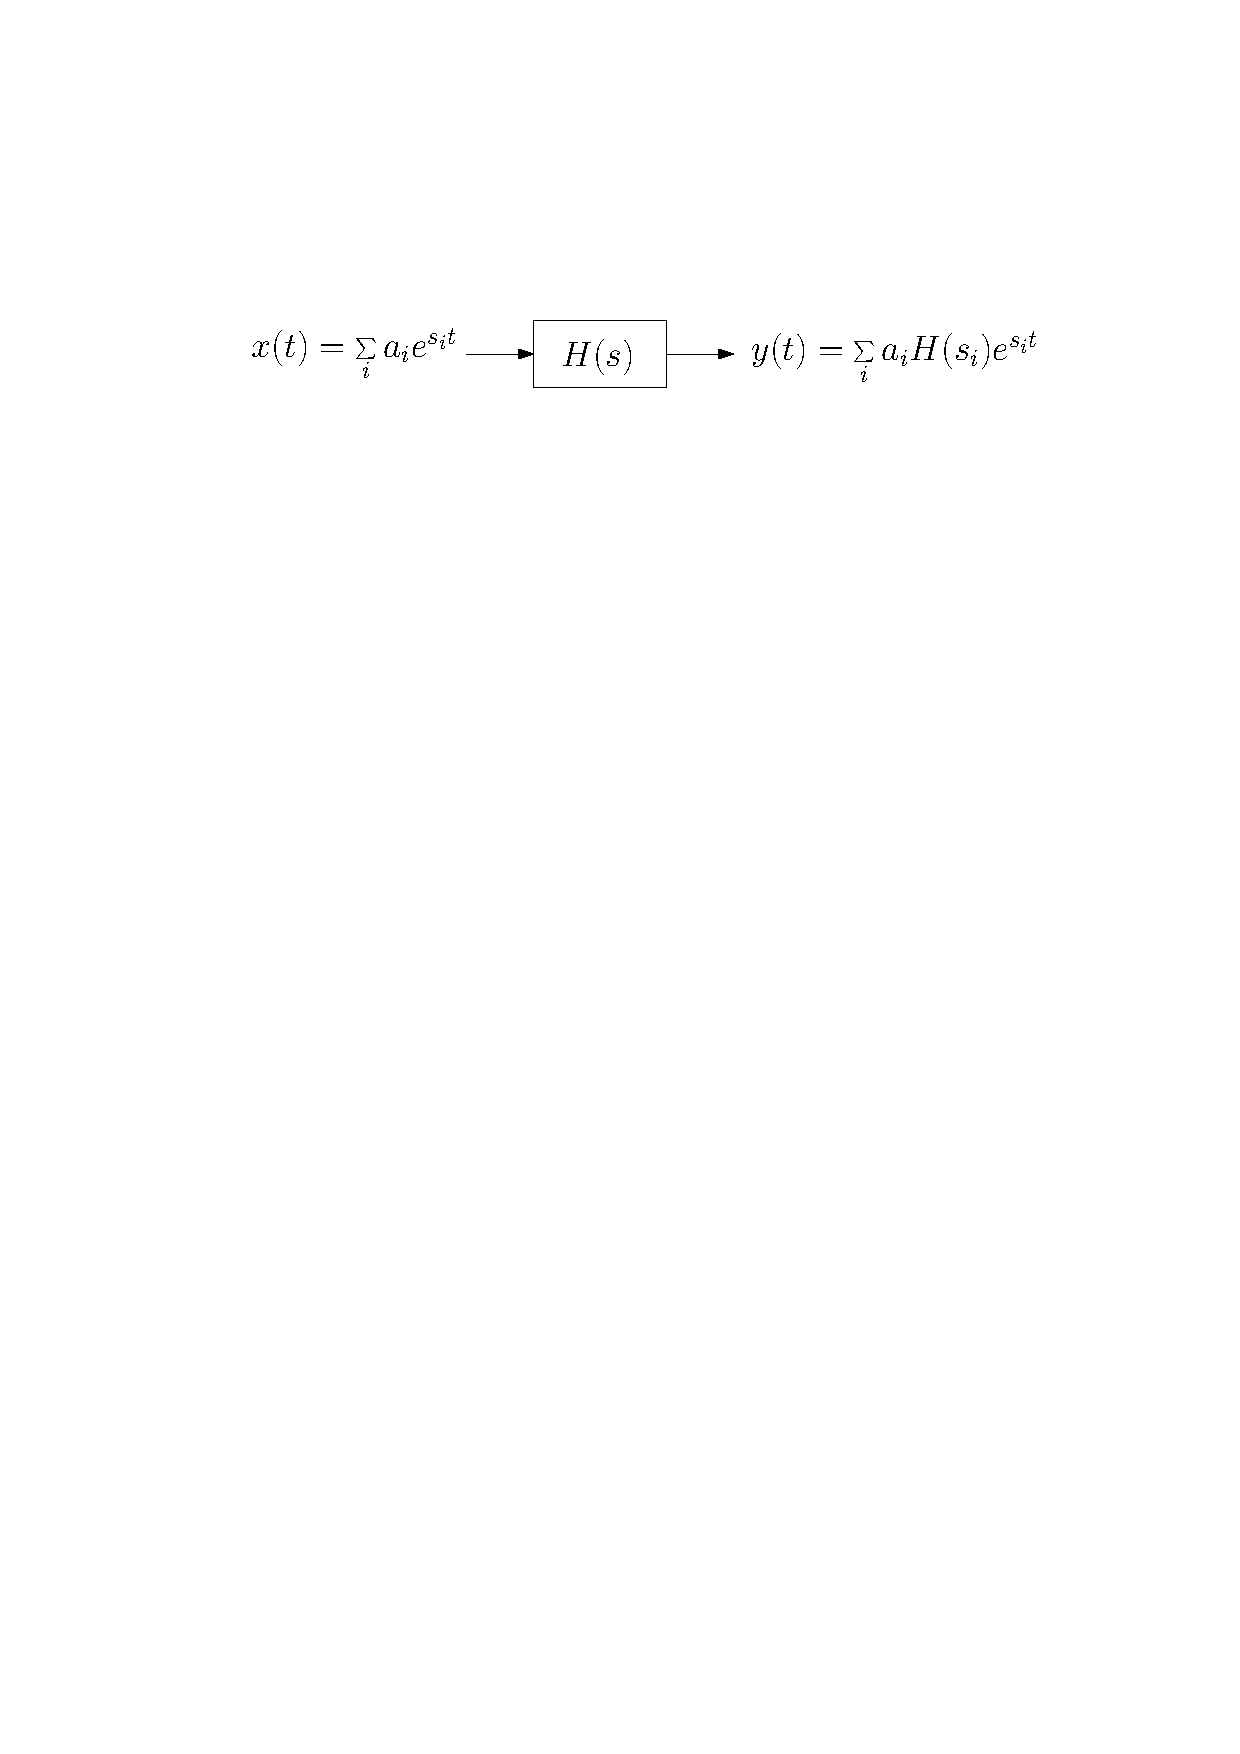
\includegraphics[scale=0.6]{graphics/ct-linear-response-complex-exp.pdf}
\end{center}
In some cases the sums are countably infinite while in others the uncountably infinite so that the sums become integrals.

\begin{example} Consider the CT system with impulse response response
  \[
  h(t) = e^{-5t}u(t)
  \]
  Determine the Eigenvalues that corresponds to the input $x(t) = \cos(t)$ and the output $y(t)$.\\

  Solution: We note the cosine can be decomposed into two complex exponentials as
  \[
  \cos(t) = \frac{1}{2}e^{jt} + \frac{1}{2}e^{-jt}
  \]
  Thus in terms of the general decomposition there are two terms with complex constants $s_1 = 0+j$ and $s_2 = 0-j$ and real constants $a_1 = a_2 = \frac{1}{2}$.
  \[
   x(t) = \sum_i a_i e^{s_it} = a_1 e^{s_1t} + a_2 e^{s_2t} = \frac{1}{2}e^{jt} + \frac{1}{2}e^{-jt} = \cos(t)
   \]
   Then the output is given by
   \[
   y(t) = \sum_i H(s_i) a_i e^{s_it} = H(s_1) a_1 e^{s_1t} + H(s_2) a_2 e^{s_2t} = H(j) \frac{1}{2}e^{jt} + H(-j)\frac{1}{2}e^{-jt}
   \]
   which requires we find the Eigenvalues $H(j)$ and $H(-j)$. To do so we use the Laplace integral
   \[
   H(j) = \int\limits_{-\infty}^{\infty}h(\tau)e^{-j\tau}\; d\tau = \int\limits_{0}^{\infty} e^{-5\tau} \, e^{-j\tau}\; d\tau = \int\limits_{0}^{\infty} e^{-(j+5)\tau}\; d\tau = \frac{-1}{j+5} e^{-(j+5)\tau} \Big|_{0}^{\infty} = \frac{1}{j+5}  
   \]
   Similarly
   \[
   H(-j) = \int\limits_{-\infty}^{\infty}h(\tau)e^{j\tau}\; d\tau = \int\limits_{0}^{\infty} e^{-5\tau} \, e^{j\tau}\; d\tau = \int\limits_{0}^{\infty} e^{-(-j+5)\tau}\; d\tau = \frac{-1}{-j+5} e^{-(j+5)\tau} \Big|_{0}^{\infty} = \frac{1}{-j+5}  
   \]
   Substituting back into the output equation gives
   \begin{align*}
     y(t) &= H(j) \frac{1}{2}e^{jt} + H(-j)\frac{1}{2}e^{-jt}\\
     &=  \frac{1}{j+5} \frac{1}{2}e^{jt} + \frac{1}{-j+5} \frac{1}{2}e^{-jt}
   \end{align*}
   We can simplify this expression using the polar form of the Eigenvalues
   \begin{align*}
     y(t) &= \frac{1}{j+5} \frac{1}{2}e^{jt} + \frac{1}{-j+5} \frac{1}{2}e^{-jt}\\
     &= Re^{j\theta} \frac{1}{2}e^{jt} + Re^{-j\theta} \frac{1}{2}e^{-jt}\\
     &= R \frac{1}{2}e^{jt + j\theta} + R \frac{1}{2}e^{-jt -j\theta}\\
     &= R\cos(t + \theta)
   \end{align*}
   where
   \[
   R = \left|\frac{1}{j+5}\right| = \frac{1}{\sqrt{26}} \mbox{ and } \theta = \angle{\frac{1}{j+5}} = -\arctan \frac{1}{5}
   \]
   Note for this system, given a sinusoidal input, the output is a scaled and phase shifted sinusoid at the same frequency, where the scaling factor and phase shift is system dependent. It is illustrative to compare this analysis to the time-domain analysis of the same impulse response and input using convolution.
   $\blacksquare$
\end{example}

\subsection{Decomposition of signals using complex exponentials}

In this course we consider the cases of stable CT systems. Recall a stable system is one in which a bounded input leads to a bounded output, or equivalently the impulse response is absolutely integrable. We will consider two decompositions of the input:

  \begin{itemize}
  \item \emph{Fourier Series}: When $x(t)$ is periodic with fundamental frequency $\omega_0$, $\Re{(s)} = 0$ so that $s = jk\omega_0$, and the decomposition is a countably infinite sum. This gives the input-output relationship
    \[
    x(t) = \sum\limits_{k = -\infty}^{\infty} a_k \, e^{j k\omega_0 t} \; \longrightarrow\; y(t) = \sum\limits_{k = -\infty}^{\infty} H(j k\omega_0)\, a_k \, e^{j k\omega_0 t}
    \]
    where $H(j k\omega_0)$ are the Eigenvalues, also called the \emph{frequency response}.
  \item \emph{Inverse Fourier Transform}: When $x(t)$ is a-periodic, $\Re{(s)} = 0$ so that $s = j\omega$, and the decomposition is an uncountably infinite sum (real integral over $\omega$). This gives the input-output relationship
    \[
    x(t) = \frac{1}{2\pi}\int\limits_{-\infty}^{\infty} X(\omega) \, e^{j \omega t}\; d\omega \;\longrightarrow\; x(t) = \frac{1}{2\pi}\int\limits_{-\infty}^{\infty} H(\omega) X(\omega) \, e^{j \omega t}\; d\omega
    \]
    where $H(j \omega)$ are the Eigenvalues, again called the \emph{frequency response}.  
  \end{itemize}

  Other courses (e.g. ECE 3704) look at the general case of unstable systems and $s \in \mathbb{C}$ with decompositions:

  \begin{itemize}
  \item \emph{One-Sided Laplace Transform}: $x(t)$ is causal and the decomposition is an uncountably infinite sum (complex integral)
  \item \emph{Two-Sided (Bilateral) Laplace Transform}: $x(t)$ is non-causal and the decomposition is an uncountably infinite sum (complex integral). This is the most general case for CT LTI systems.
  \end{itemize}

  While the Laplace decompositions require complex integration, they can be understood and computed using algebra and a table of forward transforms, which only require integration of a complex function of a real variable $t$ (this is the general approach taken in upper level courses). However, this is outside the scope of this course because of time limitations.

Instead, we will be spending the next few weeks going through the CT Fourier decompositions in some detail. You will also learn how to find the CT frequency response for a stable system, and see how to use both for analysis.

